\chapter{Parallelprogrammierung}
\section{Grundlagen}
\subsection{Coffman-Bedingungen (Deadlock-Bedingungen) \slide{54}{47}}
Wenn alle vier der folgenden Bedingungen zutreffen, liegt ein Deadlock vor.
Deadlocks können verhindert werden, indem immer mindestens eine Bedingung nicht erfüllt ist, d.h. nicht alle auf einmal erfüllt sein können.
\begin{compactenum}
	\item \textbf{Mutual exclusion}
		\begin{compactitem}
			\item beschränkter Zugriff auf eine Ressource
			\item Ressource kann nur mit einer beschränkten Anzahl von Nutzern geteilt werden
		\end{compactitem}
	\item \textbf{Hold and wait}: Warten auf alle benötigten Ressourcen, während die Kontrolle über bisher zugesprochene (mind. eine) Ressourcen behalten wird.
	\item \textbf{No preemption}: Zugewiesene Ressourcen können nur freiwillig zurückgegeben werden, die Rückgabe kann nicht erzwungen werden.
	\item \textbf{Circular Wait: }Möglichkeit von Kreisen in Ressourcen-Anfragen Graph:\\
				Zyklische Kette von Prozessen, die bereits Ressourcen (mind. eine) erhalten haben und gleichzeiig auf weitere Ressourcen warten, welche jeweils dem nächsten Prozess in der zirkulären Kette zugesprochen wurden.
\end{compactenum}

\subsection{Flynn's Taxonomy \slide{51}{13}\exRef{Grafiken von SS 14, Nr. 6}}
\todo[inline]{Grafiken korrekt? Vgl. SIMD und MISD}
\noindent\makebox[\textwidth]{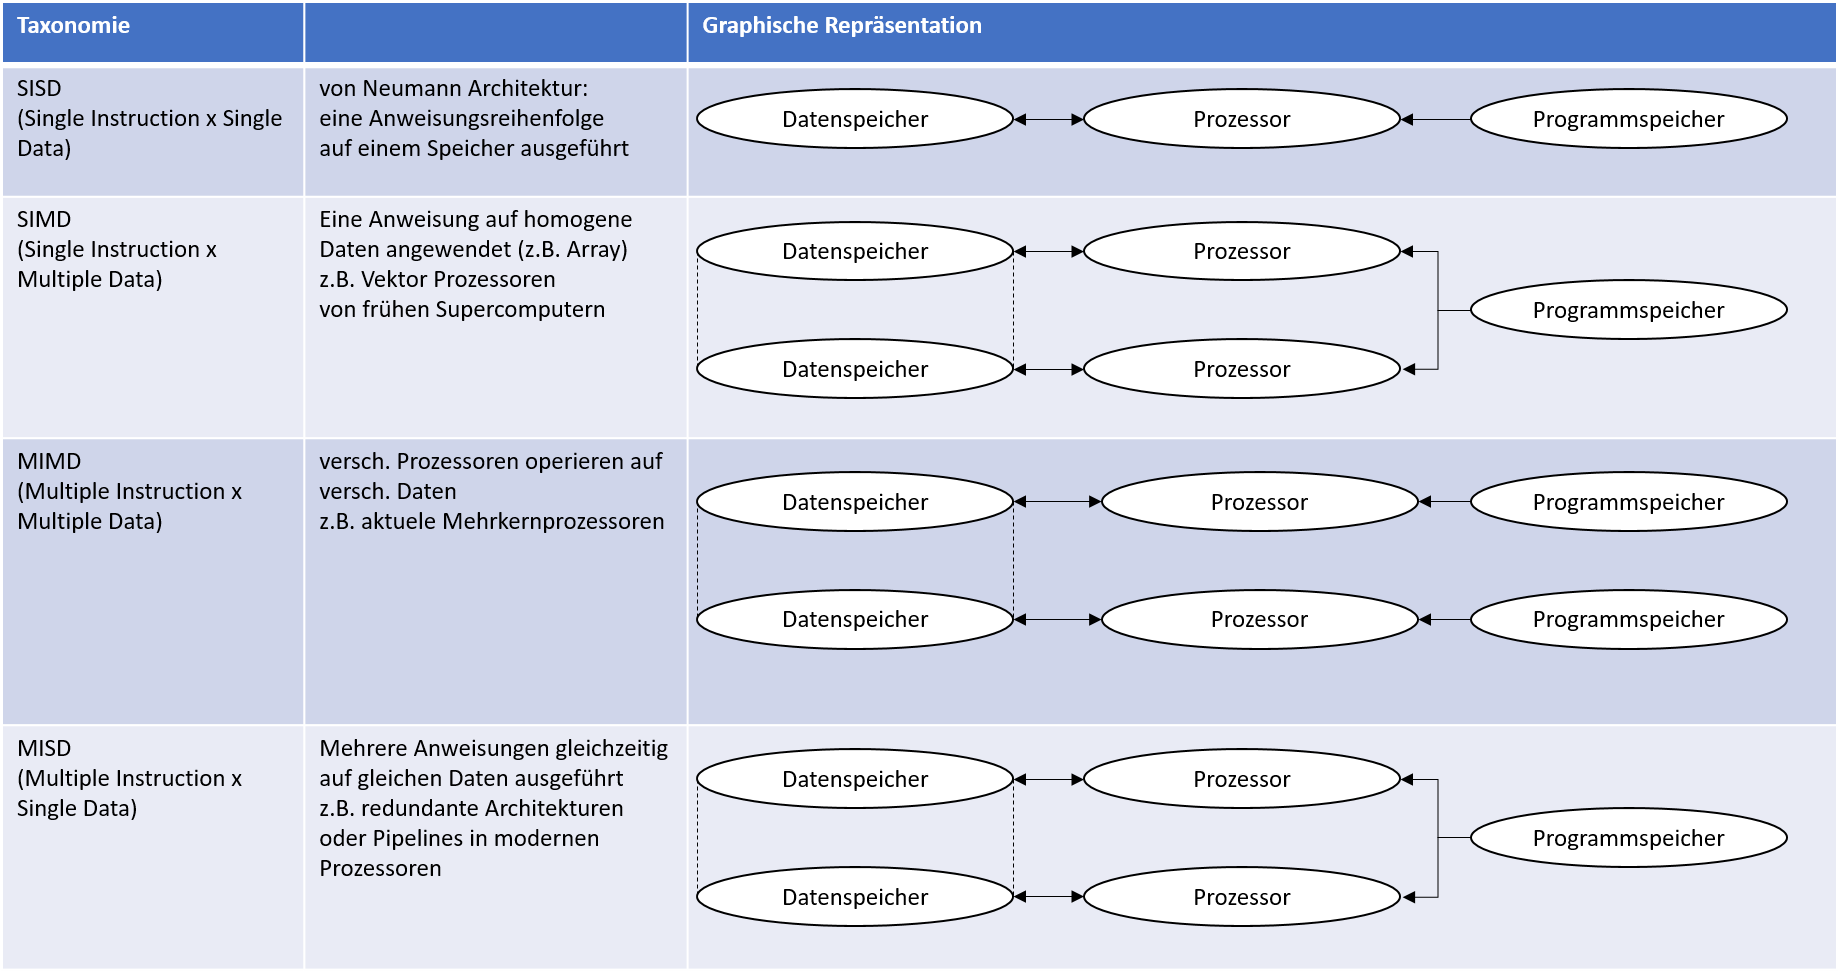
\includegraphics[width=200mm]{imgs/FlynnsTaxonomy.png}}

\subsection{Beschleunigung: Amdahl's Law \slide{51}{17}}
\myparagraph{Beschleunigung eines Algo durch die Verwendung von n Prozessoren:}
$$S(n) = \frac{T(1)}{T(n)}=\frac{\text{Ausführungszeit mit einem Prozessor}}{\text{Ausführungszeit mit n Prozessoren}}$$
\myparagraph{maximale Beschleunigung durch parallele Ausführung mit n Prozessoren:}
$$S(n)= \frac{1}{(1-p)+ \frac{p}{n}}$$
p: parallelisierbarer prozentualer Anteil des Programms

\section{MPI}
\begin{compactitem}
	\item \texttt{MPI\_Comm\_WORLD}: Standard Communicator	
	\item \texttt{MPI\_Init(\&argc, \&args)}: initialisiere MPI
	\item \texttt{MPI\_Finalize()}: Clean-Up nach Ausführung von MPI
	\item \texttt{MPI\_Comm\_rank(MPI\_Comm\_WORLD, \&my\_rank)}: my\_rank enthält den Rank des aktuellen Prozesses
	\item \texttt{MPI\_Comm\_size(MPI\_Comm\_WORLD, \&size)}: size enthält Gesamtanzahl von Prozessen
	\item \texttt{MPI\_Barrier(MPI\_Comm\_WORLD)}: Barriere, blockiert bis alle Prozesse die Barriere aufgerufen haben
	\item \texttt{MPI\_Send(void* buffer, int count, MPI\_Datatype datatype, int dest, int tag, MPI\_Comm comm)}
	\item \texttt{MPI\_Recv(void* buffer, int count, MPI\_Datatype datatype, int source, int tag, MPI\_Comm comm, MPI\_Status* status)}
\end{compactitem}

\newpage
\section{Java}
\subsection{Runnable}
\label{javaRunnable}
\lstinputlisting[language=JAVA]{codeExamples/DemoRunnable.java}

\newpage
\subsection{Callable + Feature}
\label{javaRunnable}
\lstinputlisting[language=JAVA]{codeExamples/DemoCallableFuture.java}

\newpage
\subsection{RecursiveAction / ForkJoinPool}
\label{javaRunnable}
\lstinputlisting[language=JAVA]{codeExamples/DemoRecursiveAction.java}

\newpage
\subsection{RecursiveTask / ForkJoinPool}
\label{javaRunnable}
\lstinputlisting[language=JAVA]{codeExamples/DemoRecursiveTask.java}

\subsection{AkkaActor tell()}
\label{javaRunnable}
\lstinputlisting[language=JAVA]{codeExamples/DemoAkkaActorTell.java}

\newpage
\subsection{AkkaActor ask()}
\label{javaRunnable}
\lstinputlisting[language=JAVA]{codeExamples/DemoAkkaActorAsk.java}
